%%%%%%%%%%%%%%%%%%%%%%%%%%%%%%%%%%%%%%%%%
% Journal Article
% Distributed Parallel System
% Practical 3: Comparing OpenMP scheduling
%
% Gahan M. Saraiya
% 18MCEC10
%
%%%%%%%%%%%%%%%%%%%%%%%%%%%%%%%%%%%%%%%%%
%----------------------------------------------------------------------------------------
%       PACKAGES AND OTHER DOCUMENT CONFIGURATIONS
%----------------------------------------------------------------------------------------
\documentclass[paper=letter, fontsize=12pt]{article}
\usepackage[english]{babel} % English language/hyphenation
\usepackage{amsmath,amsfonts,amsthm} % Math packages
\usepackage[utf8]{inputenc}
\usepackage{xcolor}
\usepackage{float}
\usepackage{lipsum} % Package to generate dummy text throughout this template
\usepackage{blindtext}
\usepackage{graphicx} 
\usepackage{caption}
\usepackage{subcaption}
\usepackage[sc]{mathpazo} % Use the Palatino font
\usepackage[T1]{fontenc} % Use 8-bit encoding that has 256 glyphs
\usepackage{bbding}  % to use custom itemize font
\linespread{1.05} % Line spacing - Palatino needs more space between lines
\usepackage{microtype} % Slightly tweak font spacing for aesthetics
\usepackage[hmarginratio=1:1,top=32mm,columnsep=20pt]{geometry} % Document margins
\usepackage{multicol} % Used for the two-column layout of the document
%\usepackage[hang, small,labelfont=bf,up,textfont=it,up]{caption} % Custom captions under/above floats in tables or figures
\usepackage{booktabs} % Horizontal rules in tables
\usepackage{float} % Required for tables and figures in the multi-column environment - they need to be placed in specific locations with the [H] (e.g. \begin{table}[H])
\usepackage{hyperref} % For hyperlinks in the PDF
\usepackage{lettrine} % The lettrine is the first enlarged letter at the beginning of the text
\usepackage{paralist} % Used for the compactitem environment which makes bullet points with less space between them
\usepackage{abstract} % Allows abstract customization
\renewcommand{\abstractnamefont}{\normalfont\bfseries} % Set the "Abstract" text to bold
\renewcommand{\abstracttextfont}{\normalfont\small\itshape} % Set the abstract itself to small italic text
\usepackage{titlesec} % Allows customization of titles

%Importing csv as table
\usepackage{csvsimple}

\usepackage{makecell}
\usepackage{longtable}
\renewcommand\thesection{\Roman{section}} % Roman numerals for the sections
\renewcommand\thesubsection{\Roman{subsection}} % Roman numerals for subsections
%----------------------------------------------------------------------------------------
%       DATE FORMAT
%----------------------------------------------------------------------------------------
\usepackage{datetime}
\newdateformat{monthyeardate}{\monthname[\THEMONTH], \THEYEAR}
%----------------------------------------------------------------------------------------

\titleformat{\section}[block]{\large\scshape\centering}{\thesection.}{1em}{} % Change the look of the section titles
\titleformat{\subsection}[block]{\large}{\thesubsection.}{1em}{} % Change the look of the section titles
\newcommand{\horrule}[1]{\rule{\linewidth}{#1}} % Create horizontal rule command with 1 argument of height
\usepackage{fancyhdr} % Headers and footers
\pagestyle{fancy} % All pages have headers and footers
\fancyhead{} % Blank out the default header
\fancyfoot{} % Blank out the default footer


%----------------------------------------------------------------------------------------
%       TITLE SECTION
%----------------------------------------------------------------------------------------
\title{\vspace{-15mm}\fontsize{24pt}{10pt}\selectfont\textbf{Practical 1: Speeding up performance with openmp}} % Article title
\author{
\large
{\textsc{Gahan Saraiya (18MCEC10)}}\\[2mm]
%\thanks{A thank you or further information}\\ % Your name
\normalsize \href{mailto:18mcec10@nirmauni.ac.in}{18mcec10@nirmauni.ac.in}\\[2mm] % Your email address
}
\date{}
\hypersetup{
	colorlinks=true,
	linkcolor=blue,
	filecolor=magenta,      
	urlcolor=cyan,
	pdfauthor={Gahan Saraiya},
	pdfcreator={Gahan Saraiya},
	pdfproducer={Gahan Saraiya},
}
%----------------------------------------------------------------------------------------

%----------------------------------------------------------------------------------------
%       SET HEADER AND FOOTER
%----------------------------------------------------------------------------------------
\newcommand\theauthor{Gahan Saraiya}
\newcommand\thesubject{Distributed Parallel System}
\renewcommand{\footrulewidth}{0.4pt}% default is 0pt
\fancyhead[C]{Institute of Technology, Nirma University $\bullet$ \monthyeardate\today} % Custom header text
\fancyfoot[LE,LO]{\thesubject}
\fancyfoot[RO,LE]{Page \thepage} % Custom footer text
%----------------------------------------------------------------------------------------

\usepackage[utf8]{inputenc}
\usepackage[english]{babel}
\usepackage[utf8]{inputenc}
\usepackage{fourier} 
\usepackage{array}
\usepackage{makecell}

\renewcommand\theadalign{bc}
\renewcommand\theadfont{\bfseries}
\renewcommand\theadgape{\Gape[4pt]}
\renewcommand\cellgape{\Gape[4pt]}
\newcommand*\tick{\item[\Checkmark]}
\newcommand*\arrow{\item[$\Rightarrow$]}
\newcommand*\fail{\item[\XSolidBrush]}
\usepackage{minted} % for highlighting code sytax
\definecolor{LightGray}{gray}{0.9}

\setminted[text]{
	frame=lines, 
	breaklines,
	baselinestretch=1.2,
	bgcolor=LightGray,
%	fontsize=\small
}

\setminted[python]{
	frame=lines, 
	breaklines, 
	linenos,
	baselinestretch=1.2,
%	bgcolor=LightGray,
%	fontsize=\small
}

\begin{document}
\maketitle % Insert title
\thispagestyle{fancy} % All pages have headers and footers

\section{AIM}
Write a parallel program using OpenMP to explore different impact of following scheduling. 

\section{Introduction}
OpenMP specialty is a parallelization of loops. The loop construct enables the parallelization.
\begin{minted}{c}
#pragma omp parallel for
for (...) { 
    ... 
}
\end{minted}
OpenMP then takes care about all the details of the parallelization. It creates a team of threads and distributes the iterations between the threads.

To change this behavior OpenMP provides various explicit method for scheduling listed below:
\begin{itemize}
    \item static
    \item dynamic
    \item guided
    \item auto
    \item runtime
\end{itemize}

\subsection{Explicit Scheduling}
\begin{minted}{c}
#pragma omp parallel for schedule(scheduling-type)
for (...) { 
... 
}
\end{minted}
then OpenMP uses scheduling-type for scheduling the iterations of the for loop.

\subsection{Runtime}
If the \verb|scheduling-type| (in the schedule clause of the loop construct) is equal to runtime then OpenMP determines the scheduling by the internal control variable \verb|run-sched-var|. We can set this variable by setting the environment variable \verb|OMP_SCHEDULE| to the desired scheduling type. For example, in bash-like terminals, we can do

\begin{minted}{bash}
$ export OMP_SCHEDULE=sheduling-type
\end{minted}

Another way to specify \verb|run-sched-var| is to set it with \verb|omp_set_schedule| function.

\begin{minted}{c}
...
omp_set_schedule(sheduling-type);
...
\end{minted}

\section{Explicit Scheduling in OpenMP}
\subsection{Static}
\textbf{Syntax:} \verb|schedule(static, chunk-size)|
\begin{itemize}
    \item OpenMP divides the iterations into chunks of size chunk-size and it distributes the chunks to threads in a circular order.
    \item When no \verb|chunk-size| is specified, OpenMP divides iterations into chunks that are approximately equal in size and it distributes at most one chunk to each thread.
\end{itemize}
\textbf{Example:} parallelized a for loop with $ 64 $ iterations and we used $ 4 $ threads to parallelize the for loop. Each row of stars in the examples represents a thread. Each column represents an iteration.
\subsubsection{}
\begin{minted}{c}
schedule(static):      
****************                                                
                ****************                                
                                ****************                
                                                ****************
\end{minted}
This has 16 stars in the first row. This means that the first tread executes iterations $ 1, 2, 3, \dots, 16 $. 
\\The second row has 16 blanks and then 16 stars. This means that the second thread executes iterations $ 17, 18, 19, \dots, 32$. Similar applies to the threads three and four.

\subsubsection{}
\begin{minted}{c}
schedule(static, 4):   
****            ****            ****            ****            
    ****            ****            ****            ****        
        ****            ****            ****            ****    
            ****            ****            ****            ****
\end{minted}
This divides iterations into $ 4 $ chunks of size $ 16 $ and it distributes them to $ 4 $ threads. 

\subsubsection{}
\begin{minted}{c}
schedule(static, 8):   
********                        ********                        
        ********                        ********                
                ********                        ********        
                        ********                        ********
\end{minted}
This divides iterations into $ 8 $ chunks of size $ 16 $ and it distributes them to $ 8 $ threads. 

\subsection{Dynamic}
\textbf{Syntax:} \verb|schedule(dynamic, chunk-size)|
\begin{itemize}
    \item OpenMP divides the iterations into chunks of size \verb|chunk-size|. Each thread executes a chunk of iterations and then requests another chunk until there are no more chunks available.
    \item There is no particular order in which the chunks are distributed to the threads. The order changes each time when we execute the for loop.
    \item default value for \verb|chunk-size| is $ 1 $
\end{itemize}

\subsubsection{}
\begin{minted}{c}
schedule(dynamic):
*   ** **  * * *  *      *  *    **   *  *  * *       *  *   *  
*       *     *    * *     * *   *    *        * *   *    *   
*       *    *     * *   *   *     *  *       *  *  *  *  *   *
*  *     *    * *    *  *    *    *    ** *  *   *     *   * 
\end{minted}

\subsubsection{}
\begin{minted}{c}
schedule(dynamic, 1):
    *    *     *        *   *    * *  *  *         *  * *  * *  
*  *  *   * *     *  * * *    * *      *   ***  *   *         * 
*   *  *  *  *    ** *    *      *  *  * *   *  *   *   *      
*    *     *  **        *  * *    *          *  *    *  * *  *
\end{minted}

\subsubsection{}
\begin{minted}{c}
schedule(dynamic, 4):
            ****                    ****                    ****
****            ****    ****            ****        ****        
    ****            ****    ****            ****        ****    
        ****                    ****            ****            
\end{minted}

\subsubsection{}
\begin{minted}{c}
schedule(dynamic, 8):  
                ********                                ********
                        ********        ********                
********                        ********        ********        
        ********                                                
\end{minted}

\subsection{Guided}
\textbf{Syntax:} \verb|schedule(guided, chunk-size)|

guided scheduling type is similar to the dynamic scheduling type

\begin{itemize}
    \item OpenMP again divides the iterations into chunks. Each thread executes a chunk of iterations and then requests another chunk until there are no more chunks available.
    \item The difference with the dynamic scheduling type is in the size of chunks. The size of a chunk is proportional to the number of unassigned iterations divided by the number of the threads. Therefore the size of the chunks decreases.
    \item default value for \verb|chunk-size| is $ 1 $
\end{itemize}

\subsubsection{}
\begin{minted}{c}
schedule(guided):      
                            *********                        *  
                ************                     *******  ***   
                                     *******                   *
****************                            *****       **    * 
\end{minted}

\subsubsection{}
\begin{minted}{c}
schedule(guided, 2):   
                ************                     ****     **    
                                     *******         ***    **  
                            *********                           
****************                            *****       **    **
\end{minted}

\subsubsection{}
\begin{minted}{c}
schedule(guided, 4):   
                                     *******                    
                ************                     ****    ****   
                            *********                           
****************                            *****    ****    ***
\end{minted}

\subsubsection{}
\begin{minted}{c}
schedule(guided, 8):   
                ************                 ********        ***
****************                                                
                                     ********                   
                            *********                ********
\end{minted}

The size of the chunks is decreasing. First chunk has always 16 iterations. This is because the for loop has 64 iterations and we use 4 threads to parallelize the for loop. If we divide $ \frac{64}{4} $, we get $ 16 $.

the minimum chunk size is determined in the schedule clause \verb|chunk-size|. The only exception is the last chunk. Its size might be lower then the prescribed minimum size.

The guided scheduling type is appropriate when the iterations are poorly balanced between each other. The initial chunks are larger, because they reduce overhead. The smaller chunks fills the schedule towards the end of the computation and improve load balancing. This scheduling type is especially appropriate when poor load balancing occurs toward the end of the computation.

\subsection{Auto}
\textbf{Syntax:} \verb|schedule(auto)|

The auto scheduling type delegates the decision of the scheduling to the compiler and/or runtime system.

\subsection{}
\begin{minted}{c}
schedule(auto):        
****************                                                
                ****************                                
                                ****************                
                                                ****************
\end{minted}
\section{Implementation}\label{section:implementation}
\textbf{Implementing Vector Addition}
Steps:
\begin{itemize}
	\item Implement Sequential code
	\item Implement Parallel code
	\item Implement function for verification of output (for accuracy calculation)
	\item Observe time for consumed for execution of sequential and parallel code over $ 100 $ iterations (repeating operation for $ 100 $ times)
	\item Calculate speedup for various scheduling type with input size of $ 10^6 $ \footnote{here runtime method is not actually compared and is out of scope of this experiment}
\end{itemize}

\subsection{Parallel Code}\label{code}
\inputminted{c}{../src/main.c}

\section{Analysis}
Below is the result of observation over $ 100 $ iterations for input size $ 10^6 $ for various methods

%\inputminted{text}{../src/observation.csv}

\begin{table}[!htbp]
    \centering
    \renewcommand{\arraystretch}{1.5}
    \begin{tabular}{| c | c | c |}%
        \hline
        \bfseries Method 
        & \bfseries Chunk Size 
        & \bfseries Execution Time (in seconds)
        \csvreader{../src/observation.csv}{}% use head of csv as column names
        {
            \\ \hline
            \csvcoli 
            &\csvcolii
            &\csvcoliii
        }
        \\ \hline
    \end{tabular}

    \caption{result of observation over $ 100 $ iterations for input size $ 10^6 $ for various methods}\label{table:observations}
    \medskip
    \small
    \begin{itemize}
        \item Here chunk size $ -1 $ represents that no chunk size specified in command 
        \item $ 100 $ is specified as number of fixed chunk
        \item $ 250000 $ is the value derived by $ \frac{\text{size of array}}{\text{number of threads}} $
    \end{itemize}
\end{table}

%\begin{figure}[H]
%    \centering
%    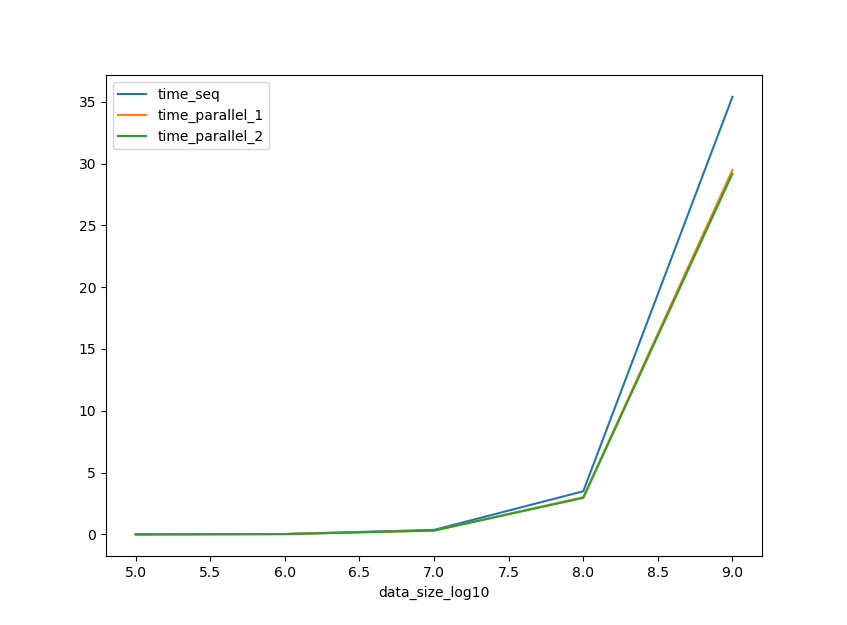
\includegraphics[width=0.8\linewidth]{assets/time_graph.png}
%    \caption{Analysis of Time consumed by thread(s) for calculation of number of inputs (x-axis scaled to the log base 10)}
%\end{figure}

\section{Conclusion}
For the example considered in Program described in Section \ref{section:implementation}.\ref{code} and results from Table \ref{table:observations} we can conclude that the task is to simply add two numbers for each index element in both the vectors.
\begin{itemize}
    \item guided scheduling method tooks minimum execution time
    \item for the dynamic scheduling the same value are updated as \verb|no-of-chunks-defined|.
\end{itemize}

\begin{table}[!htbp]
    \centering
    \begin{tabular}{c | p{15cm}}
        \textbf{Method} & \textbf{Description}
        \\ \hline \hline
        static & When \verb|schedule(static,chunk_size)| is specified, iterations are divided into chunks of size \verb|chunk_size|, and the chunks are assigned to the threads in the team in a round-robin fashion in the order of the thread number.
        
        When no \verb|chunk_size| is specified, the iteration space is divided into chunks that are approximately equal in size, and at most one chunk is distributed to each thread. The size of the chunks is unspecified in this case.
        
        A compliant implementation of the static schedule must ensure that the same assignment of logical iteration numbers to threads will be used in two loop regions if the following conditions are satisfied: 1) both loop regions have the same number of loop iterations, 2) both loop region shave the same value of \verb|chunk_size| specified, or both loop regions have \verb|nochunk_sizespecified|, 3) both loop regions bind to the same parallel region,and 4) neither loop is associated with a SIMD construct. A data dependence between the same logical iterations in two such loops is guaranteed to be satisfied allowing safe use of the no wait clause.
        \\ \hline
        dynamic & When \verb|schedule(dynamic,chunk_size)| is specified, the iterations are distributed to threads in the team in chunks. Each thread executes a chunk of iterations, then requests another chunk, until no chunks remain to be distributed.
        Each chunk contains \verb|chunk_size| iterations, except for the chunk the sequentially last iteration
        , which may have fewer iterations.When no \verb|chunk_size| is specified, it defaults to 1.
        \\ \hline
        guided & When \verb|schedule(guided,chunk_size)| is specified, the iterations are assigned to threads in the team in chunks. Each thread executes a chunk of iterations, then requests another chunk, until no chunks remain to be assigned
        For a \verb|chunk_size| of 1, the size of each chunk is proportional to the number of unassigned iterations divided by the number of threads in the team,decreasing to 1. For a \verb|chunk_size| with value k(greater than 1), the size of each chunk is determined in the same way, with the restriction that the chunks do not contain fewer thank iterations (except for the chunk that contains the sequentially last iteration, which may have fewer thank iterations).
        \\ \hline
        auto & When schedule(auto) is specified, the decision regarding scheduling is delegated to the compiler and/or runtime system. The programmer gives the implementation the freedom to choose any possible mapping of iterations to threads in the team
    \end{tabular}
\end{table}
\end{document}


\subsubsection{}